\section{Personalwesen}
\label{sec:ui-personalwesen}

\autorbeginn{Julia}

Um Raumschiffe produzieren zu können, benötigt der Spieler arbeitstüchtige Droiden, welche im Bildschirm “Personal” verwaltet werden. Dieser ist auf Abbildung \vref{img:ui-personalwesen} zu sehen.

In der oberen Hälfte des Bildschirmes sind drei verschiedene Droidentypen zu sehen, welche dem Spieler zur Verfügung sehen. Diese Typen sind in drei verschiedene Stufen unterteilt, welche jeweils in eigenen Containern dargestellt werden. Jeder Container enthält spezifische Daten zum jeweiligen Droidentyp. So wird beispielsweise der Droide Stufe eins im ersten Container beschrieben. Dabei ist ein Bild des Droiden zu sehen. Um nähere Informationen zu diesem Typ zu erhalten, steht dem Spieler ein Hilfebutton in Form eines Fragezeichens in der rechten unteren Ecke des Bildes zur Verfügung. Rot hinterlegt ist zum einen der Preis eines Droiden, welcher sich aus der später beschriebenen Datenbasis aus \vref{sub:Personal} ergibt. Daneben kann der Spieler die Anzahl der anzuheuernden Droiden auswählen. Aus der Anzahl und dem Preis der Droiden ergeben sich dann die Gesamtkosten für diese Droidenstufe. Da ein Droide monatlich gewartet werden muss, findet man die dafür anfallenden Kosten ebenfalls in dem Container zur jeweiligen Droidenstufe. Sind alle anzuheuernden Droiden ausgewählt, so kann der Spieler auf der rechten Bildschirmseite die gesamten Anheuerkosten ablesen und durch den grünen Button “Ausgewählte Droiden anheuern” den Einkauf bestätigen welches dem UseCase “Personal einstellen” entspricht.

Auf der linken unteren Hälfte des Bildschirmes befindet sich zum einen ein Container zum Ausbauen von Droiden und zum anderen einen Cointainer zum Entlassen von Droiden. Im Bereich “Ausbauen” hat der Spieler die Möglichkeit, Droiden zur Stufe 2 beziehungsweise zur Stufe 3 auszubauen. Beim Ausbauen zur nächst höheren Stufe fallen Kosten an, welche den Rot hinterlegten Textfeldern zu entnehmen sind. Rechts daneben kann die gewünschte Anzahl für den Ausbau angegeben werden. Hier hat der Spieler die Möglichkeit sich über den Hilfebutton genauer über das Ausbauen von Droiden zu informieren. Mit dem Button “Ausbau starten” wird der UseCase “Personal weiterbilden” ausgelöst. Darunter befindet sich der Bereich “Entlassen” in dem zur jeweiligen Stufe die gewünschte Anzahl an Droiden auszuwählen ist, welche entlassen werden soll. Auch hier befindet sich ein Hilfebutton für genauere Informationen. Der Button “Droiden entlassen” bestätigt die Auswahl. Dies stellt die Realisierung des UseCase “Personal entlassen” dar. 

Als weitere Informationsquelle für den Spieler dient das Liniendiagramm auf der rechten unteren Seite des Bildschirms. Hierbei werden die verfügbaren Droiden über die verschiedenen Spielrunden dargestellt. Eine Trennung der einzelnen Droidenarten wird durch unterschiedliche Linien getroffen. 

\begin{figure}[h]
  \centering
  \fbox{
    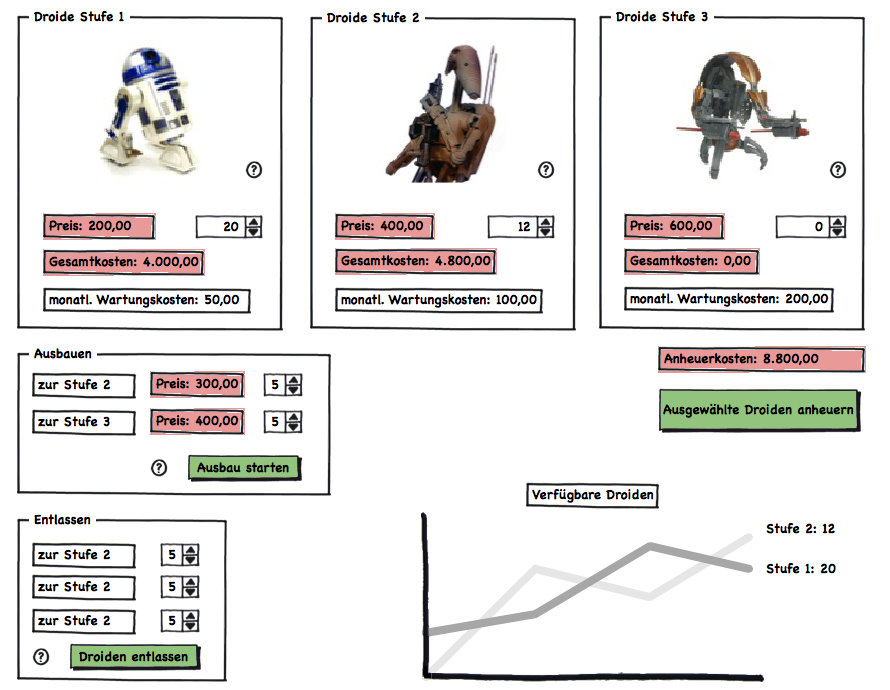
\includegraphics[width=0.9\textwidth]{40_UI/40_Personalwesen/Personalwesen.jpg}
  }
  \caption{Personalwesen}
  \label{img:ui-personalwesen}
\end{figure}

\autorende{}